\section{Fault Simulation}
\subsection{Program Counter}
\ch{is this the correct title?}
\ch{we should also show how we have modelled a fault in the heap/stack}
To simulate a single bit flip occurring in the program's execution a special fault template is introduced, illustrated in \cref{fig:faultTime}. The template selects a random value between $0$ and the maximum possible global clock value, which represents when in the programs execution a fault happens. The random value is assigned to a global variable in the UPPAAL system.\\\\
Every instruction in the Java bytecode is represented by a location, and has an associated program counter. There are edges from each location going to the locations which can be reached if one bit is flipped in the program counter. These edges have guards which check whether the time the fault is injected, corresponds to the global clock at the time the model simulation is at that particular edge. If it is, the guard will allow the edge to be traversed. There are no fault edges going back to the added locations described in \cref{subsubsec:method}, since these are not a part of the original program and therefore do not have an associated program counter.
\begin{figure}[H]
\centering
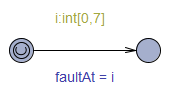
\includegraphics{figures/fault.PNG}
\caption{The UPPAAL template which selects when to perform a bit flip in the program counter}
\label{fig:faultTime}
\end{figure}\ch{update figure to use fault at between 0 and global clock}


\subsection{Opstack Complications}
Under normal execution the value of the operand stack pointer can be known at compile  time. This leaves us with two ways to simulate it, use a operand stack pointer to point at the top element or statically define the opstack element to be accessed for each instruction.

Under normal execution there is to difference between the two approaches, but then introducing fault models as PC\_Fault and INST\_Fault, it is possible to change the behaviour. This can let the operand stack pointer point to a value an instruction never would access or in the extreme case go out of bounds for the method.

Our approach is the operand stack pointer and assumes that the virtual machine will detect out of bounds. As such under a PC\_FAULT a former value of might be read instead of the current one.

The Java Virtual Machine assumes that ``There are no operand stack overflows or underflows'' \cite[c. 4.10]{java_spec} which is checked by the verifier.

\subsection{Operand Stack}
% locals and opstack
A special template selects when a fault should be introduced into the operand stack. This happens in the same way as in the program counter fault described earlier, illustrated in \cref{fig:faultTime}. The selected value is between $0$ and the maximum possible runtime of the program. \cref{fig:opstackFlip} shows how a method called \texttt{getTriesRemaining}, in which a bit flip in the operand stack occurs. Edges going back to the locations \texttt{pc0\_iconst\_2} and \texttt{pc0\_iconst\_2} are where the faults are introduced, these are added by the solution and are not a part of an unaltered model of a program. The edges have a guard, $faultTime \leq globalClock$, determined by the special template, which only allows a fault to happen if the program execution has executed for a certain amount of time. The fault itself is introduced by the update $os\lbrack osPos \rbrack\:\hat{}= 1 \ll osBitPos$, which flips bit \texttt{osBitPos} of value \texttt{osPos} in the operand stack\ch{ref to description of how we represent operand stack here?}. \texttt{osBitPos} is a random value between $0$ and $7$, which denotes which bit should be flipped. \texttt{osPos} is a random value between $0$ and the maximum size of the operand stack. After a fault has been introduced, the variable \texttt{faultTime} is set to a value higher than the maximum value of the global clock, to ensure only one fault happens per simulation.\\\\
Our approach to modelling faults in the operand stack and local variables is similar and only one of them is therefore described.
% % % % %
\begin{figure}[H]
\centering
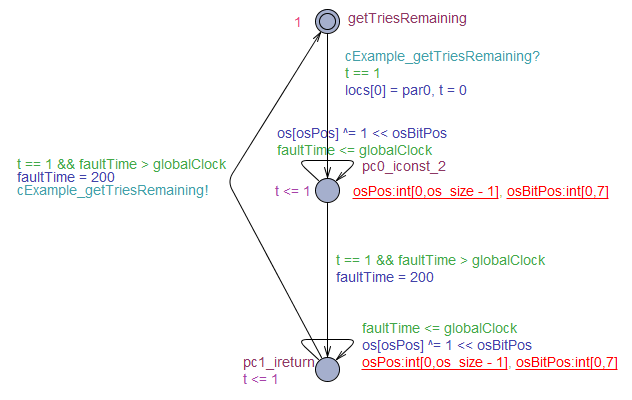
\includegraphics{figures/reportExamples/opstackRewrite.PNG}
\caption{The UPPAAL model af a method where a bit flip occurs in the operand stack.}
\label{fig:opstackFlip}
\end{figure}
\subsubsection{Instruction Fault}
\subsubsection{Heap Fault}